Viele haben lange darauf gewartet, in Eisenach hat sich erstmals am 11. Januar  2019 eine Gruppe von 12 technisch interessierten Menschen getroffen. Sie wollen sich auch zukünftig regelmä\ss ig treffen. Es soll gemeinsam gebastelt, gelötet und programmiert werden. Ihr erreicht uns über unsere Website \url{https://www.wak-lab.org} oder über unsere Whatsapp Gruppe \url{https://chat.whatsapp.com/EGc0lJaG8x9JUUz9530W5N}. Die Aktuelle Version diese FAQ findet ihr auf \url{https://github.com/thehilde/Wak-Lab-Docs/blob/master/FAQ/FAQ.pdf?raw=true}.\\
\ \\
Zunächst haben wir uns drauf verständigt diese Treffen regelmäßig in der alten Posthalterei (Abb. \ref{img:ESAPOSTHALTEREI}) abzuhalten. Dabei werden uns die Räumlichkeiten stundenweise überlassen. Au\ss erdem Treffen wir uns gelegentilch spontan im Augustiner in der Georgenstraße 30 (Abb. \ref{img:ESAAugustiner}).\\
\ \\
\begin{minipage}[t]{0.5\textwidth}
  \centering
  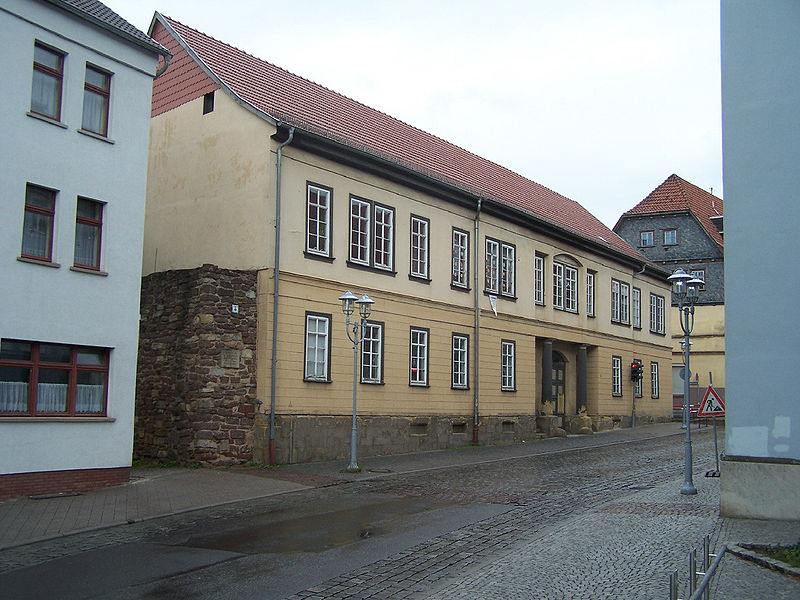
\includegraphics[height=5cm]{pictures/800px-ESAPOSTHALTEREI.jpg}
  \captionof{figure}{Alte Posthalterei}
  \label{img:ESAPOSTHALTEREI}
\end{minipage}
\begin{minipage}[t]{0.5\textwidth}
  \centering
  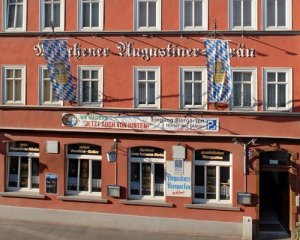
\includegraphics[height=3cm]{pictures/Augustiner.jpg}
  \captionof{figure}{Augustiner}
  \label{img:ESAAugustiner}
\end{minipage}
\ \\
\ \\
Wir wollen mit einer Präsenz in sozialen Medien und mit einem Flyer (Abb. \ref{img:FlyerMitPlatine}) zunächst andere Menschen auf unsere Idee aufmerksam machen. Das weitere Vorgehen ist von der Resonanz abhängig. Ideen über Vereinsgründung und Gemeinnützigkeit bestehen, aber wir wollen bewusst dieses Thema zunächst vertagen. \\
\ \\
\begin{minipage}[t]{0.5\textwidth}
  \centering
  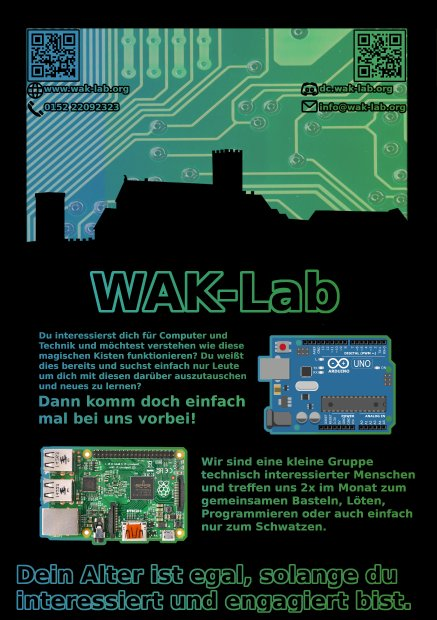
\includegraphics[height=6cm]{pictures/FlyerMitPlatine.jpg}
  \captionof{figure}{Flyer}
  \label{img:FlyerMitPlatine}
\end{minipage}
\begin{minipage}[t]{0.5\textwidth}
  \centering
  
\includegraphics[height=6cm]{pictures/FlyerRueckseite.jpg}
  \captionof{figure}{Flyer Rückseite}
  \label{img:FlyerRueckseite}
\end{minipage}

\subsection{Finanzierung}
Solange wir noch eine lose Interessensgemeinschaft sind sammeln wir bei PAYPAL \url{http://paypal.wak-lab.org} Geld für Flyer und andere notwendigen Ausgaben. Die Beteiligung ist freiwillig. Das Geld wird transparent und demokratisch ausgegeben. Eine Übersicht über die Finanzen findet ihr unter Nextcloud\textbackslash Wak-Lab\textbackslash Finanzen 2019.ods. Sachspenden die für den Betrieb der Infrastruktur benötigt werden, sind ebenso willkommen. \\
\ \\
\textbf{Hinweis:} Es versteht sich, dass Geld- und Sachspenden nach Vereinsgründung in dessen Eigentum übergeht.\\

\subsection{Abstimmungen}
Abstimmungen werden zunächst über \url{http://www.strawpoll.me} durchgeführt.\\

\begin{minipage}[t]{\textwidth}
  \centering
  
\includegraphics[height=6cm]{pictures/StrawPoll.png}
  \captionof{figure}{Online Abstimmung}
  \label{img:StrawPoll}
\end{minipage}
\subsection{Abstimmungen über einen Discord BOT}
Parallel wird getestet ob man kurzfristige Entscheidungen innerhalb einer Stunde über einen BOT im Discord realisieren kann.

\subsection{Fotos und Videos}
Grundsätzlich respektieren wir, dass jeder das Recht auf sein eigenes Foto hat. Auch wenn er in einer Gruppe zu sehen ist. Daher sollten Fotos immer angekündigt werden. Spontane Schnappschüsse sollen verifiziert werden können.\\
\ \\
In der Nextcloud gibt es einen Ordner Fotos. Dort werden die Fotos zu Freigabezwecken zwischengelagert. Soweit nichts anderes vereinbart, werden sie 24 Stunden lang von allen Mitgliedern geprüft. Dabei werden sie gelöscht, modifiziert, in den Ordner nur für internen Gebrauch oder in den Ordner zur Veröffentlichung verschoben. Nach 24 Stunden sollen die Fotos dann frühestens veröffentlicht werden. Nicht freigegebene Fotos sollen dann auch von Medien der Nutzer gelöscht werden.\ \\
\ \\
Es versteht sich, dass herabwürdigende, unangebrachte oder diffamierende Fotos gelöscht bzw. gar nicht erst zur Prüfung eingestellt werden. Unsere Gruppe legt im Interesse aller großen Wert auf die Persönlichkeitsrechte des Einzelnen.\ \\
\begin{itemize} 
\item 01\_neue Fotos
\item 02\_Nur für Mitglieder freigegebene Fotos
\item 03\_Fotos die zur Veröffentlichung vorgesehen werden
\item 04\_Fotos zur Veröffentlichung 
\end{itemize}
Innerhalb der Ordner werden die Fotos von einem Fotoadmin nach Datum in Ordner sortiert. 
\newpage


